\section{Discussion of Optical Pumping Cell Simulation Results\label{sec:discusion}}
Although it is unclear whether the FEM model is capable of accurately predicting HP $^{129}$Xe polarizations from various optical pumping cell configurations, one can discuss some qualitative results that may be applicable to the design of optical pumping cells. With the benefit of hindsight, these results are quite obvious from simple physical principals, but the visualization of gas flow, temperature and Rb distribution, and laser absorption emphasize the importance of these principals.

The first qualitative conclusion one can draw is that the distribution of Rb in the optical pumping cell body can drastically change the performance of the cell. In particular, Rb sources that are on the ``top'' and ``front'' of the cell are likely to contribute to the Rb vapor concentration to a far greater extent that Rb sources in other areas of the cell. The dominance of Rb sources on the ``top'' was observed in the 100 cc cell simulation in which the Rb source was a full-circumferential distribution (Figure \ref{fig:100ccresult}). This is due to the nature of convection transporting hot gasses to the top portion of the cell. Since the gas will be heated by the laser, the system will have a temperature gradient between the upper and lower portions of the cell. The high temperature at the upper portion of the cell will tend to evaporate Rb in those locations more quickly.

Similarly, Rb sources near the ``front'' of the cell are likely to contribute to the concentration of the Rb vapor to a far greater extent than sources in the "back" of the cell. Because the laser intensity is highest at the ``front'', gasses are likely to be close to the highest temperature experienced in the body of the cell. As seen in the initial 300 cc optical pumping cell simulation, Rb sources that are nominally in the outlet may significantly contribute to the Rb number density in the body of the cell (Figure \ref{fig:300ccrboutletresult}).

\begin{figure*}[t]
    \subfloat[The visualization of the 120 $^{\circ}$ C horizontally oriented 100 cc cell with a full-circumferential Rb distribution. The laser absorption, average temperature, and Rb polarization all show oscillatory behaviour over the 600 time-step (60 second), transient simulation. The initiation of the oscillations are preceded by a qualitative change in the convection behaviour. The orientation of the convection rotation change from axial, similar to that in figures \ref{fig:300ccrboutletresult} and \ref{fig:results300ccresult}, to transverse, as shown above. Once established, this new convection behavior does not appear to revert back to the previous pattern. The oscillations are driven by the interchange of positive feedback, when laser heated gasses vaporize excess Rb, and negative feedback, when the excess Rb block laser light at the front of the cell so that it can no longer effectively heat the gas. \label{fig:100ccresult}]{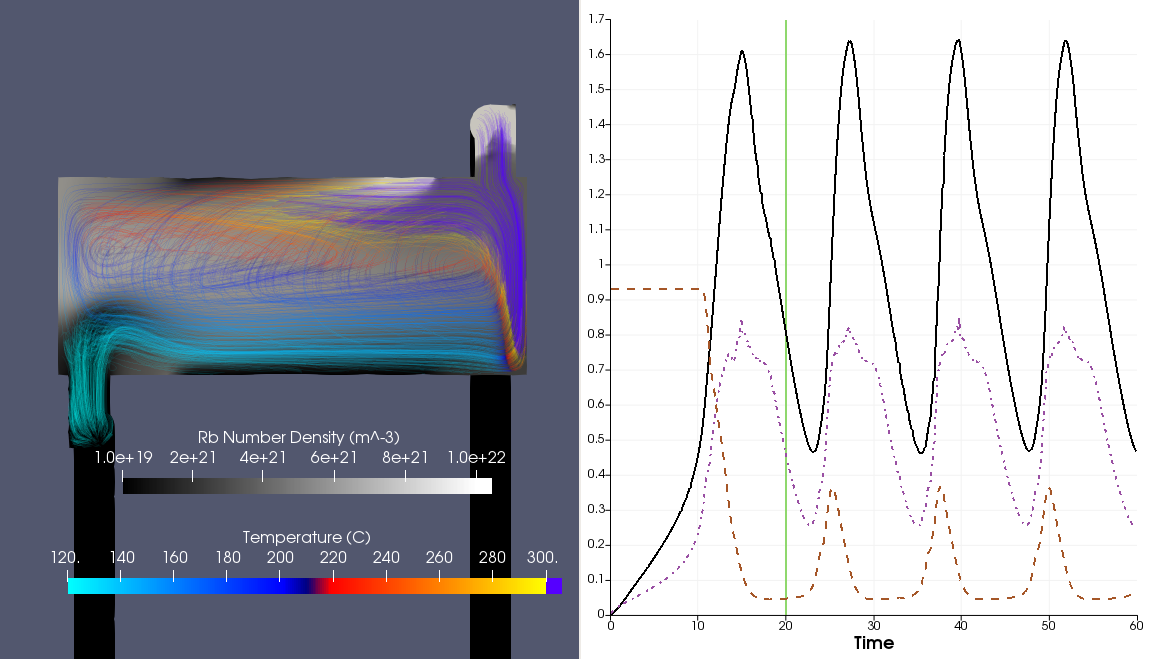
\includegraphics[width=0.3\textwidth]{Figures/120CFull.png}}\rulesep
    \subfloat[The visualization of the initial 140 $^{\circ}$ C, 300 cc cell with a Rb drop as the source and the Rb film in the outlet extending up to the wall of the body of the cell. When heated by exiting gasses, the Rb film in the outlet can diffuse back into the body of the cell and block the laser. In the simulation, this caused the sharp decline in Rb polarization at time-step 69 (6.9 seconds). body.\label{fig:300ccrboutletresult}]{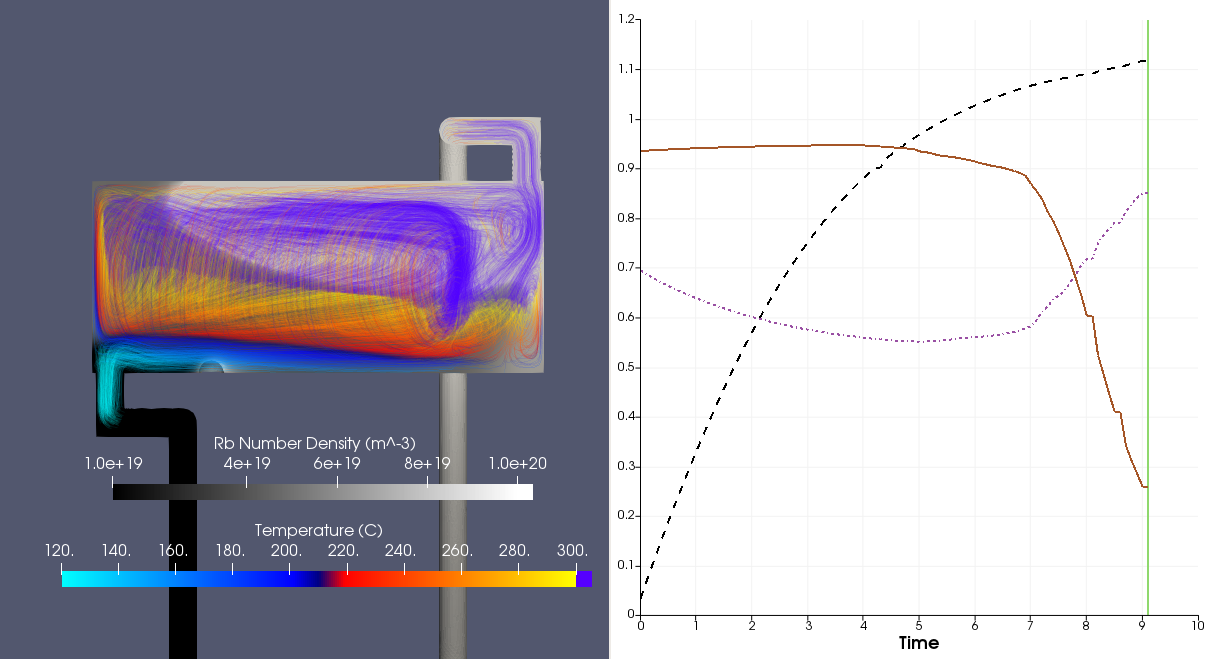
\includegraphics[width=0.33\textwidth]{Figures/300cc140crboutletnolegend.png}}\rulesep
    \subfloat[The visualization of the 130 $^{\circ}$C, 300 cc cell with a Rb drop as the source as the Rb film in the outlet moved to the first bend in the outlet. Although moving the Rb film in the outlet farther from the body prevents diffusion back into the cell body, as in figure \ref{fig:300ccrboutletresult}, the heated gasses exiting through the outlet still evolve an excess amount of Rb. In the simulations, the excess Rb number density at some locations in the outlet was approximately one order of magnitude greater than the Rb number density in the cell body. Although not confirmed by these simulations, that could result in rapid depolarization of the HP $^{129}$Xe in the outlet.   \label{fig:results300ccresult}]{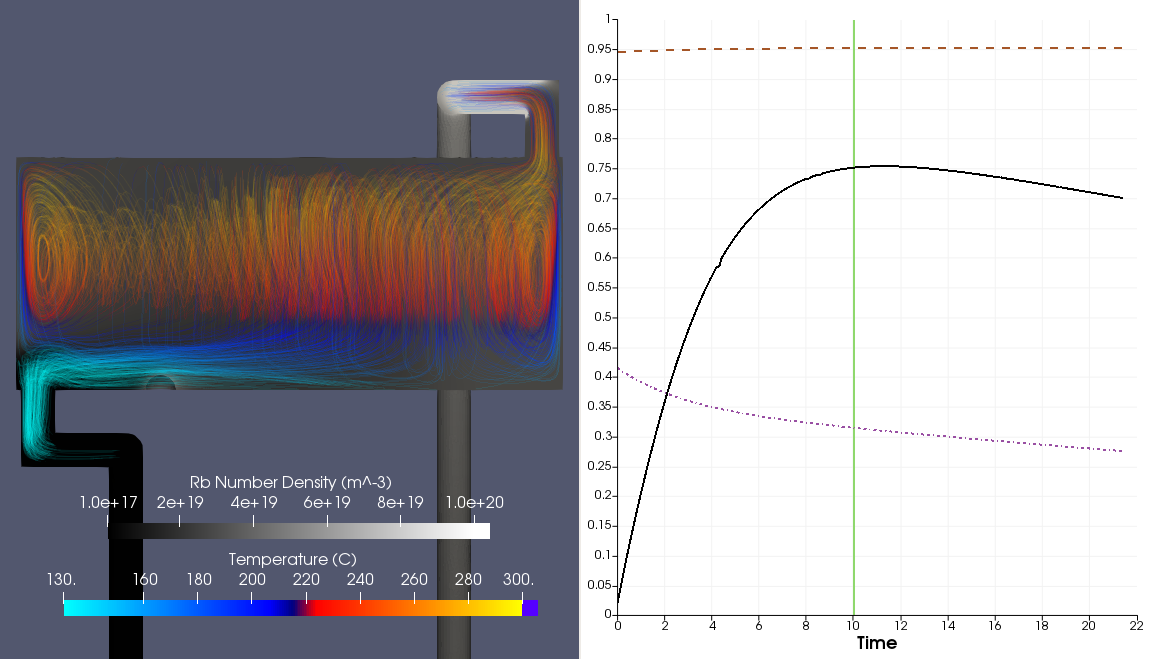
\includegraphics[width=0.3\textwidth]{Figures/130CDrop.png}}
    \caption{Three visualizations of the simulations. On the right of each subfigure is a visualization of the optical pumping cell with gas flow streamlines. The color of the streamlines denotes the temperature of the gas in $^{\circ}$C. Temperatures above 300 $^{\circ}$C are shown in purple. The geometry of the cell is sliced, and the color of the slice denotes the number density of Rb in inverse cubic meters. On the left of each subfigure is a graph of the average temperature in fraction above the set point temperature (black dashed), fraction of laser power absorbed(dotted purple), and fraction of Rb polarization(solid brown). The green vertical line in each graph denotes the time step at which the visualization on the right is taken.}
    \label{fig:resultvisualization}
\end{figure*}

Depending on the configuration of the Rb in the cell, light may be absorbed preferentially at the front of the cell causing large dark regions in the body. Although not definitively observed in these simulations, such a situation could give rise to decreased $^{129}$Xe polarization.

A final qualitative conclusion that may be drawn from the currents model is the importance of Rb in the outlet of the optical pumping cell. Rb films in the outlet which are near the cell body may contribute to the Rb density in the body of the cell. Also importantly, the Rb number density in the outlet of the cell may be significantly higher than the Rb number density in the body(Figure \ref{fig:results300ccresult}). The Rb vapor in the outlet will not be polarized and, thus, may give rise to rapid depolarization of HP$^{129}$Xe passing through the outlet. However, this rapid depolarization was not definitively observed in these simulations.